\documentclass[bibliography=totoc, a4paper, 12pt]{article}
\usepackage[utf8]{inputenc}
\usepackage[russian]{babel}
\usepackage{hyperref}
\usepackage{graphicx}
% \usepackage{csquotes}
\usepackage[nottoc,notlot,notlof]{tocbibind}
\usepackage{icomma}
\hypersetup{
    colorlinks,
    allcolors=blue
}
\usepackage{longtable, moreverb}
\usepackage{ amssymb, latexsym, amsmath, amsthm}
\newtheorem{myth}{Теорема}
\newtheorem{mylm}{Лемма}
\newtheorem*{myco}{Следствие}
\usepackage{verbatim}
\newcommand{\rol} {\textrm{rol}}
\newcommand{\pphi}[1] {P^{\delta}(\varphi_{#1})}
\textwidth=18cm       % Эти строки нужны для того,
\textheight=21cm      % чтобы равенства уместились
\oddsidemargin=-1cm % на странице

\sloppy

\xdef\LastDeclaredEncoding{T2A}
% Переносы математики.
\begingroup
\catcode`\+\active\gdef+{\mathchar8235\nobreak\discretionary{}{\usefont{OT1}{cmr}{m}{n}\char43}{}}
\catcode`\-\active\gdef-{\mathchar8704\nobreak\discretionary{}{\usefont{OMS}{cmsy}{m}{n}\char0}{}}
\catcode`\=\active\gdef={\mathchar12349\nobreak\discretionary{}{\usefont{OT1}{cmr}{m}{n}\char61}{}}
\catcode`\<\active\gdef<{\mathchar"313C\nobreak\discretionary{}{\usefont{OML}{cmm}{m}{n}\char60}{}}
\catcode`\>\active\gdef>{\mathchar"313E\nobreak\discretionary{}{\usefont{OML}{cmm}{m}{n}\char62}{}}
\endgroup
\def\times{\mathchar8706\nobreak\discretionary{}{\usefont{OMS}{cmsy}{m}{n}\char2}{}}
\def\subset{\mathchar"321A\nobreak\discretionary{}{\usefont{OMS}{cmsy}{m}{n}\char26}{}}
%\supset,\subseteq,\notin
\def\supset{\mathchar"321B\nobreak\discretionary{}{\usefont{OMS}{cmsy}{m}{n}\char27}{}}
\def\subseteq{\mathchar"3212\nobreak\discretionary{}{\usefont{OMS}{cmsy}{m}{n}\char18}{}}
\def\neq{\not=\nobreak\discretionary{}{\usefont{OMS}{cmsy}{m}{n}\char54\usefont{OT1}{cmr}{m}{n}\char61}{}}
\def\sim{\mathchar"3218\nobreak\discretionary{}{\usefont{OMS}{cmsy}{m}{n}\char24}{}}
\def\in{\mathchar"3232\nobreak\discretionary{}{\usefont{OMS}{cmsy}{m}{n}\char50}{}}
\def\to{\mathchar"3221\nobreak\discretionary{}{\usefont{OMS}{cmsy}{m}{n}\char33}{}}
\def\?#1{#1\nobreak\discretionary{}{\hbox{$\mathsurround=0pt #1$}}{}}
% Конец переносов математики.

\begin{document}
% Восстанавливаем после amsmath.
\begingroup \catcode`\"=12
\gdef\newmcodes@{\mathcode`\'39\mathcode`\*42\mathcode`\."613A%
\mathcode`\-"8000\mathcode`\/47\mathcode`\:"603A\relax}%
\endgroup
\mathcode`\=="8000 \mathcode`\+="8000 \mathcode`\-="8000
\mathcode`\<="8000 \mathcode`\>="8000

% \tableofcontents

% \newpage

\setcounter{secnumdepth}{-1}

\section{Введение}
Одним из стандартных способов задания функций k\nobreakdash-значной логики являются поляризованные полиномиальные формы (ППФ),
которые также называются обобщенными формами Рида-Мюллера, или каноническими поляризованными полиномами. В ППФ каждая переменная
имеет определенную поляризацию. Длиной полиномиальной формы называется число попарно различных слагаемых в ней. Длиной функции
$F$ в классе ППФ называется наименьшая длина среди длин всех поляризованных полиномиальных форм, реализующих $F$.
Функция Шеннона $L^K_k(n)$ длины определяется как наибольшая длина среди всех функций $k$\nobreakdash-значной логики в классе $K$
от~$n$~переменных, если $K$ опущено, то подразумевается класс ППФ.
Практическое применение ППФ нашли при построении программируемых логических матриц (ПЛМ)~\cite{ue04, sb90}, сложность ПЛМ
напрямую зависит от длины ППФ, по которой она построена. Поэтому в ряде работ исследуется сложность ППФ различных функций.

В 1993  В.\,П.\,Супрун~\cite{sv93} получил первые оценки функции Шеннона для функций алгебры логики :
$$
L_2(n) \geqslant C_n^{[\frac{n}{2}]},
$$
$$
L_2(n) < 3 \cdot 2^{n-1}.
$$
где [$a$] обозначает целую часть $a$.

Точное значение функции Шеннона для функций алгебры логики в 1995\,г. было
найдено Н.\,А.\,Перязевым~\cite{pn95} :
$$
L_2(n) = \left[\frac{2^{n+1}}{3}\right].
$$

Функции $k$\nobreakdash-значных логик являются естественным обобщением функций алгебры логики.
Для функций $k$\nobreakdash-значной логики верхняя оценка функции Шеннона была получена в 2002\,г. С.\,Н.\,Селезневой~\cite{ss02} :
$$
L_k(n) < \frac{k(k-1)}{k(k-1)+1}k^n.
$$

При построении ПЛМ рассматривают и другие полиномиальные формы. Например класс обобщенных полиномиальных форм.
В классе обобщенных полиномиальных форм, в отличие от класса поляризованных полиномиальных форм, переменные могут иметь
различную поляризацию в разных слагаемых. В статье К.\,Д.\,Кириченко~\cite{kk05}, опубликованной в 2005\,г., получена верхняя оценка
функции Шеннона в классе обобщенных полиномиальных форм функций алгебры логики :
$$
L^{\text{О.П.}}_2(n) < \frac{2 ^ {n + 1}(\log_2n+1)}{n}.
$$

Верхняя оценка функции Шеннона в классе обобщенных полиномиальных форм функций k\nobreakdash-значной логики была получена
С.\,Н.\,Селезневой А.\,Б.\,Дайняком в 2008\,г.~\cite{sd08}:
$$
L^{\text{О.П.}}_k(n) \lesssim 2\cdot\frac{k ^ n}{n}\cdot \ln n \text{ при } n \rightarrow \infty.
$$

В 2012\,г. Н.\,К.\,Маркеловым была получена нижняя оценка функции Шеннона для функции трехзначной логики в классе
поляризованных полиномов~\cite{mn12}:
$$
L_3(n) \geqslant \left[\frac{3}{4}3^n\right].
$$

\section{Основные определения}

Пусть $k \geqslant 2$ -- натуральное число,
$E_k = \{0, 1, \dots, k - 1\}$
. Весом набора
$\alpha = (a_1, \dots, a_n ) \in E_k^n$ назовем число $|\alpha| = \sum\limits_{i=1}^n a_i$.
Моном $\prod\limits_{a_i\neq0}x_i^{a_i}$ назовем соответствующим набору $\alpha = (a_1, \dots, a_n ) \in E_k^n$ и обозначим
через $K_{\alpha}$. По определению положим, что константа 1 соответствует набору из всех нулей.
Функцией $k$\nobreakdash-значной логики называется отображение $f^{(n)} : E_k^n \rightarrow E_k$,
$n = 0, 1, \dots$ . Множество всех $k$\nobreakdash-значных функций обозначим через $P_k$ , множество
всех $k$\nobreakdash-значных функций, зависящих от переменных $x_1, \dots, x_n$ , обозначим через $P_k^n$ .

Если $k$ -- простое число, то каждая функция $k$\nobreakdash-значной логики $f(x_1 , \dots , x_n)$
может быть однозначно задана формулой вида

$$ f(x_1, \dots, x_n) = \sum_{\alpha \in E_k^n:c_f(\alpha) \neq 0}c_f(\alpha)K_\alpha \; ,$$
где $c_f(\alpha) \in E_k$ -- коэффициенты, $\alpha \in E_k$, и операции сложения и умножения
рассматриваются по модулю $k$. Это представление функций $k$\nobreakdash-значной
логики называется ее полиномом по модулю $k$. При простых $k$ однозначно
определенный полином по модулю k для функции $k$\nobreakdash-значной логики $f$ будем
обозначать через $P(f)$.

Определим поляризованные полиномиальные формы по модулю $k$. Поляризованной переменной $x_i$ с поляризацией $d$,
$d \in E_k$ , назовем выражение вида $(x_i + d)$. Поляризованным мономом по вектору поляризации $\delta$,
$\delta = (d_1, \dots, d_n) \in E_k^n$, назовем произведение вида $(x_{i_1} + d_{i_1} )^{m_1}\cdots(x_{i_r} + d_{i_r})^{m_r}$,
где $1 \leqslant i_1 < \ldots < i_r \leqslant n$, и $1 \leqslant m 1 , \dots , m_r \leqslant k - 1$. Обычный моном является
мономом, поляризованным по вектору $\tilde{0} = (0, \dots, 0) \in E_k^n $

Выражение вида $\sum\limits_{i=1}^lc_i \cdot K_i$, где $c_i \in E_k\setminus\{0\}$ -- коэффициенты, $K_i$ -- попарно
различные мономы, поляризованные по вектору $\delta = (d_1, \dots, d_n) \in E_k^n$, $i = 1, \dots , l$, назовем
поляризованной полиномиальной нормальной формой (ППФ) по вектору поляризации $\delta$. Мы будем считать, что константа 0
является ППФ по произвольному вектору поляризации. Заметим, что при простых $k$ для каждого вектора поляризации каждую функцию
$k$\nobreakdash-значной логики можно однозначно представить ППФ по этому вектору поляризации \cite{ss02}. При простых $k$
однозначно определенную ППФ по вектору поляризации $\delta \in E_k^n$ для функции
$f \in P_k^n$ будем обозначать через $P^{\delta}(f)$.

Длиной $l(p)$ ППФ $p$ назовем число попарно различных слагаемых в этой
ППФ. Положим, что $l(0) = 0$. При простых $k$ длиной функции $k$\nobreakdash-значной
логики в классе ППФ называется величина $l^{\text{ППФ}}(f) = \min\limits_{\delta \in E_k^n}l(P^{\delta}(f))$.

Сложностью системы ППФ, имеющих один и тот же вектор поляризации, называется число попарно различных слагаемых,
встречающихся во всех этих ППФ. При простых $k$ сложностью $L_k^{\text{ППФ}}(F)$ системы функций $k$\nobreakdash-значной
логики $F = \{f_1(x_1 , \dots , x_n ), \dots , f_m (x_1 , \dots , x_n )\}$ в классе ППФ называется минимальная сложность
среди всех таких систем ППФ $\{p_1 , \dots , p_m \}$, что все ППФ $p_1 , \dots , p_m$ имеют один и тот же вектор поляризации,
и ППФ $p_j$ реализует функцию $f_j,\; j = 1, \dots , m$. Понятно, что для произвольной системы функций $k$\nobreakdash-значной
логики $F = \{f_1(x_1, \dots, x_n), \dots , f_m(x_1 , \dots , x_n )\}$ верна оценка $L_k^{\text{ППФ}}(F) \leqslant k^n$.

Пусть $k$ -- простое число, и $A_k \subseteq P_k$ , а $A^n_k = A_k \cap P_k^n$ . Введем функцию
Шеннона $L^{\text{ППФ}}_{A_k}(m, n)$ сложности систем функций $k$\nobreakdash-значной логики, принадлежащих множеству $A$,
в классе ППФ:
$$L^{\text{ППФ}}_{A_k}(m, n) = \max_{B\subseteq A_k^n, |B|=m}L^{\text{ППФ}}_{k}(B) .$$

Если $A_k = P_k$ , то функцию Шеннона будем обозначать через $L^{\text{ППФ}}_{A_k}(m, n)$.

Функция $k$\nobreakdash-значной логики $f(x_1 ,\dots , x_n)$ называется симметрической, если
$$f(\pi(x_1), \dots, \pi(x_n)) = f(x_1, \dots, x_n)$$
для произвольной перестановки $\pi$ на множестве переменных $\{x_1 , \dots , x_n \}$.
Множество всех симметрических функций $k$\nobreakdash-значной логики обозначим через $S_k$.
Симметрическая функция $f(x_1, \dots, x_n)$ называется периодической c
периодом $\tau = (\tau_0 \tau_1 \dots \tau_{T-1}) \in E_k^T$ , если $f(\alpha) = \tau_j$ при $|\alpha| = j(\mod T)$
для каждого набора $\alpha \in E_k^n$. При этом число $T$ называется длиной периода. Периодическую функцию
$k$\nobreakdash-значной логики $f(x_1 , \dots , x_n)$ с периодом $\tau = (\tau_0 \tau_1 \dots \tau_{T-1}) \in E_k^T$
будем обозначать через $f^{(n)}_{(\tau_0 \tau_1 \dots \tau_{T-1})}$. Понятно, что
такое обозначение полностью определяет эту функцию.

Введем функцию $\rol(\alpha, i) \in E_k^n \times E_k \rightarrow E_k^n$, производящую чиклический сдвиг вектора $\alpha$
влево. Пусть $\alpha = (a_1, \dots, a_n)$, тогда $\rol(\alpha, i) = (a_{(1+i)\mod k}, \dots, a_{(n+i)\mod k})$.

Класс функций $A$ называется вырожденным, если при $n \rightarrow \infty$ для любой функции
${f_n \in A_n}$ выполняется: $l(f_n) = \overline{o}(5^n)$.

В данной работе рассматривается класс функций $\mathcal{A}$, состоящий из всех линейных комбинаций
функций $f$ и $g$, где $f$ -- это периодическая симметрическая функция с периодом (1,1,4,4), а
\mbox{$g$ -- это} периодическая симметрическая функция с периодом (1,4,4,1). А также его подкласс
$\mathcal{F}$ состоящий из следующих четырех функций: $f,g,f+g,f+4g$.

\section{Результаты}
\subsection{Поляризованные полиномы для функций из класса $\mathcal{A}$}

\begin{myth} При $n \geqslant 1 $ для периодических функций пятизначной логики $f_n = f^{\left(n\right)}_{\left(1144\right)}$,
$g_n = f^{\left(n\right)}_{\left(1441\right)}$ верны следующие равенства:
$$\begin{array}{l}
 f_{n+1} = j_0(x_{n+1})f_n + j_1(x_{n+1})g_n + 4\,j_2(x_{n+1})f_n + 4\,j_3(x_{n+1})g_n + j_4(x_{n+1})f_n =\\
4 \, f_{n} x_{n+1}^{4} + {\left(3 \, f_{n} + 2 \, g_{n}\right)} x_{n+1}^{3} + 3 \, {\left(f_{n} + g_{n}\right)} x_{n+1}^{2} + {\left(4 \, f_{n} + g_{n}\right)} x_{n+1} + f_{n}=\\
4 \, f_{n} {\left(x_{n+1} + 1\right)}^{4} + 2 \, {\left(f_{n} + g_{n}\right)} {\left(x_{n+1} + 1\right)}^{3} + {\left(3 \, f_{n} + 2 \, g_{n}\right)} {\left(x_{n+1} + 1\right)}^{2} + {\left(f_{n} + g_{n}\right)} {\left(x_{n+1} + 1\right)} + f_{n}=\\
4 \, f_{n} {\left(x_{n+1} + 2\right)}^{4} + {\left(f_{n} + 2 \, g_{n}\right)} {\left(x_{n+1} + 2\right)}^{3} + {\left(f_{n} + g_{n}\right)} {\left(x_{n+1} + 2\right)}^{2} + 3 \, g_{n} {\left(x_{n+1} + 2\right)} + 4 \, g_{n}=\\
4 \, f_{n} {\left(x_{n+1} + 3\right)}^{4} + 2 \, g_{n} {\left(x_{n+1} + 3\right)}^{3} + 2 \, f_{n} {\left(x_{n+1} + 3\right)}^{2} + 2 \, g_{n} {\left(x_{n+1} + 3\right)} + 4 \, f_{n}=\\
4 \, f_{n} {\left(x_{n+1} + 4\right)}^{4} + 2 \, {\left(2 \, f_{n} + g_{n}\right)} {\left(x_{n+1} + 4\right)}^{3} + {\left(f_{n} + 4 \, g_{n}\right)} {\left(x_{n+1} + 4\right)}^{2} + 3 \, g_{n} {\left(x_{n+1} + 4\right)} + g_{n}=\\
\end{array}$$
\end{myth}

\begin{proof}

Первое равенство следует из теоремы 1.

При поляризации $x_{n+1}$, когда $d_{n+1} = 0$
$$\begin{array}{l}
f_{n+1}(\bar{x}_n, 0) = 0 + 0 + 0 + 0 + f_n = f_n \\
f_{n+1}(\bar{x}_n, 1) = 4\,f_n + 3\,f_n + 2\,g_n + 3\,f_n + 3\,g_n + 4\,f_n + g_n + f_n = g_n \\
f_{n+1}(\bar{x}_n, 2) = 4\,f_n + 4\,f_n + g_n + 2\,f_n + 2\,g_n + 3\,f_n + 2\,g_n + f_n = 4\,f_n \\
f_{n+1}(\bar{x}_n, 3) = 4\,f_n + f_n + 4\,g_n + 2\,f_n + 2\,g_n + 2\,f_n + 3\,g_n + f_n = 4\,g_n \\
f_{n+1}(\bar{x}_n, 4) = 4\,f_n + 2\,f_n + 3\,g_n + 3\,f_n + 3\,g_n + f_n + 4\,g_n + f_n = f_n \\
\end{array}$$
При поляризации $x_{n+1}$, когда $d_{n+1} = 1$
$$\begin{array}{l}
f_{n+1}(\bar{x}_n, 0) = 4\,f_n + 2\,f_n + 2\,g_n + 3\,f_n + 2\,g_n + f_n + g_n + f_n = f_n \\
f_{n+1}(\bar{x}_n, 1) = 4\,f_n + f_n + g_n + 2\,f_n + 3\,g_n + 2\,f_n + 2\,g_n + f_n = g_n \\
f_{n+1}(\bar{x}_n, 2) = 4\,f_n + 4\,f_n + 4\,g_n + 2\,f_n + 3\,g_n + 3\,f_n + 3\,g_n + f_n = 4\,f_n \\
f_{n+1}(\bar{x}_n, 3) = 4\,f_n + 3\,f_n + 3\,g_n + 3\,f_n + 2\,g_n + 4\,f_n + 4\,g_n + f_n = 4\,g_n \\
f_{n+1}(\bar{x}_n, 4) = 0 + 0 + 0 + 0 + f_n = f_n \\
\end{array}$$
При поляризации $x_{n+1}$, когда $d_{n+1} = 2$
$$\begin{array}{l}
f_{n+1}(\bar{x}_n, 0) = 4\,f_n + 3\,f_n + g_n + 4\,f_n + 4\,g_n + g_n + 4\,g_n = f_n \\
f_{n+1}(\bar{x}_n, 1) = 4\,f_n + 2\,f_n + 4\,g_n + 4\,f_n + 4\,g_n + 4\,g_n + 4\,g_n = g_n \\
f_{n+1}(\bar{x}_n, 2) = 4\,f_n + 4\,f_n + 3\,g_n + f_n + g_n + 2\,g_n + 4\,g_n = 4\,f_n \\
f_{n+1}(\bar{x}_n, 3) = 0 + 0 + 0 + 0 + 4\,g_n = 4\,g_n \\
f_{n+1}(\bar{x}_n, 4) = 4\,f_n + f_n + 2\,g_n + f_n + g_n + 3\,g_n + 4\,g_n = f_n \\
\end{array}$$
При поляризации $x_{n+1}$, когда $d_{n+1} = 3$
$$\begin{array}{l}
f_{n+1}(\bar{x}_n, 0) = 4\,f_n + 4\,g_n + 3\,f_n + g_n + 4\,f_n = f_n \\
f_{n+1}(\bar{x}_n, 1) = 4\,f_n + 3\,g_n + 2\,f_n + 3\,g_n + 4\,f_n = g_n \\
f_{n+1}(\bar{x}_n, 2) = 0 + 0 + 0 + 0 + 4\,f_n = 4\,f_n \\
f_{n+1}(\bar{x}_n, 3) = 4\,f_n + 2\,g_n + 2\,f_n + 2\,g_n + 4\,f_n = 4\,g_n \\
f_{n+1}(\bar{x}_n, 4) = 4\,f_n + g_n + 3\,f_n + 4\,g_n + 4\,f_n = f_n \\
\end{array}$$
При поляризации $x_{n+1}$, когда $d_{n+1} = 4$
$$\begin{array}{l}
f_{n+1}(\bar{x}_n, 0) = 4\,f_n + f_n + 3\,g_n + f_n + 4\,g_n + 2\,g_n + g_n = f_n \\
f_{n+1}(\bar{x}_n, 1) = 0 + 0 + 0 + 0 + g_n = g_n \\
f_{n+1}(\bar{x}_n, 2) = 4\,f_n + 4\,f_n + 2\,g_n + f_n + g_n + 3\,g_n + g_n = 4\,f_n \\
f_{n+1}(\bar{x}_n, 3) = 4\,f_n + 2\,f_n + g_n + 4\,f_n + g_n + g_n + g_n = 4\,g_n \\
f_{n+1}(\bar{x}_n, 4) = 4\,f_n + 3\,f_n + 4\,g_n + 4\,f_n + g_n + 4\,g_n + g_n = f_n \\
\end{array}$$

\end{proof}

\begin{myth} При $n \geqslant 1 $ для периодических функций пятизначной логики $f_n = f^{\left(n\right)}_{\left(1144\right)}$,
$g_n = f^{\left(n\right)}_{\left(1441\right)}$ верны следующие равенства:
$$\begin{array}{l}
 g_{n+1} = j_0(x_{n+1})g_n + 4\,j_1(x_{n+1})f_n + 4\,j_2(x_{n+1})g_n + j_3(x_{n+1})f_n + j_4(x_{n+1})g_n=\\
4 \, g_{n} x_{n+1}^{4} + 3 \, {\left(f_{n} + g_{n}\right)} x_{n+1}^{3} + {\left(2 \, f_{n} + 3 \, g_{n}\right)} x_{n+1}^{2} + 4 \, {\left(f_{n} + g_{n}\right)} x_{n+1} + g_{n}=\\
4 \, g_{n} {\left(x_{n+1} + 1\right)}^{4} + {\left(3 \, f_{n} + 2 \, g_{n}\right)} {\left(x_{n+1} + 1\right)}^{3} + 3 \, {\left(f_{n} + g_{n}\right)} {\left(x_{n+1} + 1\right)}^{2} + {\left(4 \, f_{n} + g_{n}\right)} {\left(x_{n+1} + 1\right)} + g_{n}=\\
4 \, g_{n} {\left(x_{n+1} + 2\right)}^{4} + {\left(3 \, f_{n} + g_{n}\right)} {\left(x_{n+1} + 2\right)}^{3} + {\left(4 \, f_{n} + g_{n}\right)} {\left(x_{n+1} + 2\right)}^{2} + 2 \, f_{n} {\left(x_{n+1} + 2\right)} + f_{n}=\\
4 \, g_{n} {\left(x_{n+1} + 3\right)}^{4} + 3 \, f_{n} {\left(x_{n+1} + 3\right)}^{3} + 2 \, g_{n} {\left(x_{n+1} + 3\right)}^{2} + 3 \, f_{n} {\left(x_{n+1} + 3\right)} + 4 \, g_{n}=\\
4 \, g_{n} {\left(x_{n+1} + 4\right)}^{4} + {\left(3 \, f_{n} + 4 \, g_{n}\right)} {\left(x_{n+1} + 4\right)}^{3} + {\left(f_{n} + g_{n}\right)} {\left(x_{n+1} + 4\right)}^{2} + 2 \, f_{n} {\left(x_{n+1} + 4\right)} + 4 \, f_{n}=\\
\end{array}$$
\end{myth}

\begin{proof}

Первое равенство следует из теоремы 1.

При поляризации $x_{n+1}$, когда $d_{n+1} = 0$
$$\begin{array}{l}
g_{n+1}(\bar{x}_n, 0) = 0 + 0 + 0 + 0 + g_n = g_n \\
g_{n+1}(\bar{x}_n, 1) = 4\,g_n + 3\,f_n + 3\,g_n + 2\,f_n + 3\,g_n + 4\,f_n + 4\,g_n + g_n = 4\,f_n \\
g_{n+1}(\bar{x}_n, 2) = 4\,g_n + 4\,f_n + 4\,g_n + 3\,f_n + 2\,g_n + 3\,f_n + 3\,g_n + g_n = 4\,g_n \\
g_{n+1}(\bar{x}_n, 3) = 4\,g_n + f_n + g_n + 3\,f_n + 2\,g_n + 2\,f_n + 2\,g_n + g_n = f_n \\
g_{n+1}(\bar{x}_n, 4) = 4\,g_n + 2\,f_n + 2\,g_n + 2\,f_n + 3\,g_n + f_n + g_n + g_n = g_n \\
\end{array}$$
При поляризации $x_{n+1}$, когда $d_{n+1} = 1$
$$\begin{array}{l}
g_{n+1}(\bar{x}_n, 0) = 4\,g_n + 3\,f_n + 2\,g_n + 3\,f_n + 3\,g_n + 4\,f_n + g_n + g_n = g_n \\
g_{n+1}(\bar{x}_n, 1) = 4\,g_n + 4\,f_n + g_n + 2\,f_n + 2\,g_n + 3\,f_n + 2\,g_n + g_n = 4\,f_n \\
g_{n+1}(\bar{x}_n, 2) = 4\,g_n + f_n + 4\,g_n + 2\,f_n + 2\,g_n + 2\,f_n + 3\,g_n + g_n = 4\,g_n \\
g_{n+1}(\bar{x}_n, 3) = 4\,g_n + 2\,f_n + 3\,g_n + 3\,f_n + 3\,g_n + f_n + 4\,g_n + g_n = f_n \\
g_{n+1}(\bar{x}_n, 4) = 0 + 0 + 0 + 0 + g_n = g_n \\
\end{array}$$
При поляризации $x_{n+1}$, когда $d_{n+1} = 2$
$$\begin{array}{l}
g_{n+1}(\bar{x}_n, 0) = 4\,g_n + 4\,f_n + 3\,g_n + f_n + 4\,g_n + 4\,f_n + f_n = g_n \\
g_{n+1}(\bar{x}_n, 1) = 4\,g_n + f_n + 2\,g_n + f_n + 4\,g_n + f_n + f_n = 4\,f_n \\
g_{n+1}(\bar{x}_n, 2) = 4\,g_n + 2\,f_n + 4\,g_n + 4\,f_n + g_n + 3\,f_n + f_n = 4\,g_n \\
g_{n+1}(\bar{x}_n, 3) = 0 + 0 + 0 + 0 + f_n = f_n \\
g_{n+1}(\bar{x}_n, 4) = 4\,g_n + 3\,f_n + g_n + 4\,f_n + g_n + 2\,f_n + f_n = g_n \\
\end{array}$$
При поляризации $x_{n+1}$, когда $d_{n+1} = 3$
$$\begin{array}{l}
g_{n+1}(\bar{x}_n, 0) = 4\,g_n + f_n + 3\,g_n + 4\,f_n + 4\,g_n = g_n \\
g_{n+1}(\bar{x}_n, 1) = 4\,g_n + 2\,f_n + 2\,g_n + 2\,f_n + 4\,g_n = 4\,f_n \\
g_{n+1}(\bar{x}_n, 2) = 0 + 0 + 0 + 0 + 4\,g_n = 4\,g_n \\
g_{n+1}(\bar{x}_n, 3) = 4\,g_n + 3\,f_n + 2\,g_n + 3\,f_n + 4\,g_n = f_n \\
g_{n+1}(\bar{x}_n, 4) = 4\,g_n + 4\,f_n + 3\,g_n + f_n + 4\,g_n = g_n \\
\end{array}$$
При поляризации $x_{n+1}$, когда $d_{n+1} = 4$
$$\begin{array}{l}
g_{n+1}(\bar{x}_n, 0) = 4\,g_n + 2\,f_n + g_n + f_n + g_n + 3\,f_n + 4\,f_n = g_n \\
g_{n+1}(\bar{x}_n, 1) = 0 + 0 + 0 + 0 + 4\,f_n = 4\,f_n \\
g_{n+1}(\bar{x}_n, 2) = 4\,g_n + 3\,f_n + 4\,g_n + f_n + g_n + 2\,f_n + 4\,f_n = 4\,g_n \\
g_{n+1}(\bar{x}_n, 3) = 4\,g_n + 4\,f_n + 2\,g_n + 4\,f_n + 4\,g_n + 4\,f_n + 4\,f_n = f_n \\
g_{n+1}(\bar{x}_n, 4) = 4\,g_n + f_n + 3\,g_n + 4\,f_n + 4\,g_n + f_n + 4\,f_n = g_n \\
\end{array}$$

\end{proof}

\begin{myth} При $n \geqslant 1 $ для периодических функций пятизначной логики $f_n = f^{\left(n\right)}_{\left(1144\right)}$,
$g_n = f^{\left(n\right)}_{\left(1441\right)}$ верны следующие равенства:
$$\begin{array}{l}
s_{n+1}^1 = f_{n+1} + g_{n+1}=\\
 {\left(4 \, f_{n} + 4 \, g_{n}\right)} x^{4} + f_{n} x^{3} + g_{n} x^{2} + 3 \, f_{n} x + f_{n} + g_{n} =\\
 {\left(4 \, f_{n} + 4 \, g_{n}\right)} {\left(x + 1\right)}^{4} + 4 \, g_{n} {\left(x + 1\right)}^{3} + f_{n} {\left(x + 1\right)}^{2} + 2 \, g_{n} {\left(x + 1\right)} + f_{n} + g_{n} =\\
 {\left(4 \, f_{n} + 4 \, g_{n}\right)} {\left(x + 2\right)}^{4} + {\left(4 \, f_{n} + 3 \, g_{n}\right)} {\left(x + 2\right)}^{3} + 2 \, g_{n} {\left(x + 2\right)}^{2} + {\left(2 \, f_{n} + 3 \, g_{n}\right)} {\left(x + 2\right)} + f_{n} + 4 \, g_{n} =\\
 {\left(4 \, f_{n} + 4 \, g_{n}\right)} {\left(x + 3\right)}^{4} + {\left(3 \, f_{n} + 2 \, g_{n}\right)} {\left(x + 3\right)}^{3} + 2 \, {\left(f_{n} + g_{n}\right)} {\left(x + 3\right)}^{2} + {\left(3 \, f_{n} + 2 \, g_{n}\right)} {\left(x + 3\right)} + 4 \, f_{n} + 4 \, g_{n} =\\
 {\left(4 \, f_{n} + 4 \, g_{n}\right)} {\left(x + 4\right)}^{4} + {\left(2 \, f_{n} + g_{n}\right)} {\left(x + 4\right)}^{3} + 2 \, f_{n} {\left(x + 4\right)}^{2} + {\left(2 \, f_{n} + 3 \, g_{n}\right)} {\left(x + 4\right)} + 4 \, f_{n} + g_{n} =\\
 \end{array}$$
\end{myth}

 \begin{proof}

Первое равенство следует из теоремы 1.

При поляризации $x_{n+1}$, когда $d_{n+1} = 0$
$$\begin{array}{l}
s_{n+1}^1(\bar{x}_n, 0) = 0 + 0 + 0 + 0 + f_n + g_n = f_n + g_n \\
s_{n+1}^1(\bar{x}_n, 1) = 4\,f_n + 4\,g_n + f_n + g_n + 3\,f_n + f_n + g_n = 4\,f_n + g_n \\
s_{n+1}^1(\bar{x}_n, 2) = 4\,f_n + 4\,g_n + 3\,f_n + 4\,g_n + f_n + f_n + g_n = 4\,f_n + 4\,g_n \\
s_{n+1}^1(\bar{x}_n, 3) = 4\,f_n + 4\,g_n + 2\,f_n + 4\,g_n + 4\,f_n + f_n + g_n = f_n + 4\,g_n \\
s_{n+1}^1(\bar{x}_n, 4) = 4\,f_n + 4\,g_n + 4\,f_n + g_n + 2\,f_n + f_n + g_n = f_n + g_n \\
\end{array}$$
При поляризации $x_{n+1}$, когда $d_{n+1} = 1$
$$\begin{array}{l}
s_{n+1}^1(\bar{x}_n, 0) = 4\,f_n + 4\,g_n + 4\,g_n + f_n + 2\,g_n + f_n + g_n = f_n + g_n \\
s_{n+1}^1(\bar{x}_n, 1) = 4\,f_n + 4\,g_n + 2\,g_n + 4\,f_n + 4\,g_n + f_n + g_n = 4\,f_n + g_n \\
s_{n+1}^1(\bar{x}_n, 2) = 4\,f_n + 4\,g_n + 3\,g_n + 4\,f_n + g_n + f_n + g_n = 4\,f_n + 4\,g_n \\
s_{n+1}^1(\bar{x}_n, 3) = 4\,f_n + 4\,g_n + g_n + f_n + 3\,g_n + f_n + g_n = f_n + 4\,g_n \\
s_{n+1}^1(\bar{x}_n, 4) = 0 + 0 + 0 + 0 + f_n + g_n = f_n + g_n \\
\end{array}$$
При поляризации $x_{n+1}$, когда $d_{n+1} = 2$
$$\begin{array}{l}
s_{n+1}^1(\bar{x}_n, 0) = 4\,f_n + 4\,g_n + 2\,f_n + 4\,g_n + 3\,g_n + 4\,f_n + g_n + f_n + 4\,g_n = f_n + g_n \\
s_{n+1}^1(\bar{x}_n, 1) = 4\,f_n + 4\,g_n + 3\,f_n + g_n + 3\,g_n + f_n + 4\,g_n + f_n + 4\,g_n = 4\,f_n + g_n \\
s_{n+1}^1(\bar{x}_n, 2) = 4\,f_n + 4\,g_n + f_n + 2\,g_n + 2\,g_n + 3\,f_n + 2\,g_n + f_n + 4\,g_n = 4\,f_n + 4\,g_n \\
s_{n+1}^1(\bar{x}_n, 3) = 0 + 0 + 0 + 0 + f_n + 4\,g_n = f_n + 4\,g_n \\
s_{n+1}^1(\bar{x}_n, 4) = 4\,f_n + 4\,g_n + 4\,f_n + 3\,g_n + 2\,g_n + 2\,f_n + 3\,g_n + f_n + 4\,g_n = f_n + g_n \\
\end{array}$$
При поляризации $x_{n+1}$, когда $d_{n+1} = 3$
$$\begin{array}{l}
s_{n+1}^1(\bar{x}_n, 0) = 4\,f_n + 4\,g_n + f_n + 4\,g_n + 3\,f_n + 3\,g_n + 4\,f_n + g_n + 4\,f_n + 4\,g_n = f_n + g_n \\
s_{n+1}^1(\bar{x}_n, 1) = 4\,f_n + 4\,g_n + 2\,f_n + 3\,g_n + 2\,f_n + 2\,g_n + 2\,f_n + 3\,g_n + 4\,f_n + 4\,g_n = 4\,f_n + g_n \\
s_{n+1}^1(\bar{x}_n, 2) = 0 + 0 + 0 + 0 + 4\,f_n + 4\,g_n = 4\,f_n + 4\,g_n \\
s_{n+1}^1(\bar{x}_n, 3) = 4\,f_n + 4\,g_n + 3\,f_n + 2\,g_n + 2\,f_n + 2\,g_n + 3\,f_n + 2\,g_n + 4\,f_n + 4\,g_n = f_n + 4\,g_n \\
s_{n+1}^1(\bar{x}_n, 4) = 4\,f_n + 4\,g_n + 4\,f_n + g_n + 3\,f_n + 3\,g_n + f_n + 4\,g_n + 4\,f_n + 4\,g_n = f_n + g_n \\
\end{array}$$
При поляризации $x_{n+1}$, когда $d_{n+1} = 4$
$$\begin{array}{l}
s_{n+1}^1(\bar{x}_n, 0) = 4\,f_n + 4\,g_n + 3\,f_n + 4\,g_n + 2\,f_n + 3\,f_n + 2\,g_n + 4\,f_n + g_n = f_n + g_n \\
s_{n+1}^1(\bar{x}_n, 1) = 0 + 0 + 0 + 0 + 4\,f_n + g_n = 4\,f_n + g_n \\
s_{n+1}^1(\bar{x}_n, 2) = 4\,f_n + 4\,g_n + 2\,f_n + g_n + 2\,f_n + 2\,f_n + 3\,g_n + 4\,f_n + g_n = 4\,f_n + 4\,g_n \\
s_{n+1}^1(\bar{x}_n, 3) = 4\,f_n + 4\,g_n + f_n + 3\,g_n + 3\,f_n + 4\,f_n + g_n + 4\,f_n + g_n = f_n + 4\,g_n \\
s_{n+1}^1(\bar{x}_n, 4) = 4\,f_n + 4\,g_n + 4\,f_n + 2\,g_n + 3\,f_n + f_n + 4\,g_n + 4\,f_n + g_n = f_n + g_n \\
\end{array}$$

\end{proof}

\begin{myth} При $n \geqslant 1 $ для периодических функций пятизначной логики $f_n = f^{\left(n\right)}_{\left(1144\right)}$,
$g_n = f^{\left(n\right)}_{\left(1441\right)}$ верны следующие равенства:
$$\begin{array}{l}
s_{n+1}^2 = f_{n+1} + 2\,g_{n+1}=\\
 {\left(4 \, f_{n} + 3 \, g_{n}\right)} x^{4} + {\left(4 \, f_{n} + 3 \, g_{n}\right)} x^{3} + {\left(2 \, f_{n} + 4 \, g_{n}\right)} x^{2} + {\left(2 \, f_{n} + 4 \, g_{n}\right)} x + f_{n} + 2 \, g_{n} =\\
 {\left(4 \, f_{n} + 3 \, g_{n}\right)} {\left(x + 1\right)}^{4} + {\left(3 \, f_{n} + g_{n}\right)} {\left(x + 1\right)}^{3} + {\left(4 \, f_{n} + 3 \, g_{n}\right)} {\left(x + 1\right)}^{2} + {\left(4 \, f_{n} + 3 \, g_{n}\right)} {\left(x + 1\right)} + f_{n} + 2 \, g_{n} =\\
 {\left(4 \, f_{n} + 3 \, g_{n}\right)} {\left(x + 2\right)}^{4} + {\left(2 \, f_{n} + 4 \, g_{n}\right)} {\left(x + 2\right)}^{3} + {\left(4 \, f_{n} + 3 \, g_{n}\right)} {\left(x + 2\right)}^{2} + {\left(4 \, f_{n} + 3 \, g_{n}\right)} {\left(x + 2\right)} + 2 \, f_{n} + 4 \, g_{n} =\\
 {\left(4 \, f_{n} + 3 \, g_{n}\right)} {\left(x + 3\right)}^{4} + {\left(f_{n} + 2 \, g_{n}\right)} {\left(x + 3\right)}^{3} + 2 \, {\left(f_{n} + 2 \, g_{n}\right)} {\left(x + 3\right)}^{2} + {\left(f_{n} + 2 \, g_{n}\right)} {\left(x + 3\right)} + 4 \, f_{n} + 3 \, g_{n} =\\
 {\left(4 \, f_{n} + 3 \, g_{n}\right)} {\left(x + 4\right)}^{4} + {\left(3 \, f_{n} + g_{n}\right)} {\left(x + 4\right)}^{2} + {\left(4 \, f_{n} + 3 \, g_{n}\right)} {\left(x + 4\right)} + 3 \, f_{n} + g_{n} =\\
 \end{array}$$
\end{myth}

 \begin{proof}

Первое равенство следует из теоремы 1.

При поляризации $x_{n+1}$, когда $d_{n+1} = 0$
$$\begin{array}{l}
s_{n+1}^2(\bar{x}_n, 0) = 0 + 0 + 0 + 0 + f_n + 2\,g_n = f_n + 2\,g_n \\
s_{n+1}^2(\bar{x}_n, 1) = 4\,f_n + 3\,g_n + 4\,f_n + 3\,g_n + 2\,f_n + 4\,g_n + 2\,f_n + 4\,g_n + f_n + 2\,g_n = 3\,f_n + g_n \\
s_{n+1}^2(\bar{x}_n, 2) = 4\,f_n + 3\,g_n + 2\,f_n + 4\,g_n + 3\,f_n + g_n + 4\,f_n + 3\,g_n + f_n + 2\,g_n = 4\,f_n + 3\,g_n \\
s_{n+1}^2(\bar{x}_n, 3) = 4\,f_n + 3\,g_n + 3\,f_n + g_n + 3\,f_n + g_n + f_n + 2\,g_n + f_n + 2\,g_n = 2\,f_n + 4\,g_n \\
s_{n+1}^2(\bar{x}_n, 4) = 4\,f_n + 3\,g_n + f_n + 2\,g_n + 2\,f_n + 4\,g_n + 3\,f_n + g_n + f_n + 2\,g_n = f_n + 2\,g_n \\
\end{array}$$
При поляризации $x_{n+1}$, когда $d_{n+1} = 1$
$$\begin{array}{l}
s_{n+1}^2(\bar{x}_n, 0) = 4\,f_n + 3\,g_n + 3\,f_n + g_n + 4\,f_n + 3\,g_n + 4\,f_n + 3\,g_n + f_n + 2\,g_n = f_n + 2\,g_n \\
s_{n+1}^2(\bar{x}_n, 1) = 4\,f_n + 3\,g_n + 4\,f_n + 3\,g_n + f_n + 2\,g_n + 3\,f_n + g_n + f_n + 2\,g_n = 3\,f_n + g_n \\
s_{n+1}^2(\bar{x}_n, 2) = 4\,f_n + 3\,g_n + f_n + 2\,g_n + f_n + 2\,g_n + 2\,f_n + 4\,g_n + f_n + 2\,g_n = 4\,f_n + 3\,g_n \\
s_{n+1}^2(\bar{x}_n, 3) = 4\,f_n + 3\,g_n + 2\,f_n + 4\,g_n + 4\,f_n + 3\,g_n + f_n + 2\,g_n + f_n + 2\,g_n = 2\,f_n + 4\,g_n \\
s_{n+1}^2(\bar{x}_n, 4) = 0 + 0 + 0 + 0 + f_n + 2\,g_n = f_n + 2\,g_n \\
\end{array}$$
При поляризации $x_{n+1}$, когда $d_{n+1} = 2$
$$\begin{array}{l}
s_{n+1}^2(\bar{x}_n, 0) = 4\,f_n + 3\,g_n + f_n + 2\,g_n + f_n + 2\,g_n + 3\,f_n + g_n + 2\,f_n + 4\,g_n = f_n + 2\,g_n \\
s_{n+1}^2(\bar{x}_n, 1) = 4\,f_n + 3\,g_n + 4\,f_n + 3\,g_n + f_n + 2\,g_n + 2\,f_n + 4\,g_n + 2\,f_n + 4\,g_n = 3\,f_n + g_n \\
s_{n+1}^2(\bar{x}_n, 2) = 4\,f_n + 3\,g_n + 3\,f_n + g_n + 4\,f_n + 3\,g_n + f_n + 2\,g_n + 2\,f_n + 4\,g_n = 4\,f_n + 3\,g_n \\
s_{n+1}^2(\bar{x}_n, 3) = 0 + 0 + 0 + 0 + 2\,f_n + 4\,g_n = 2\,f_n + 4\,g_n \\
s_{n+1}^2(\bar{x}_n, 4) = 4\,f_n + 3\,g_n + 2\,f_n + 4\,g_n + 4\,f_n + 3\,g_n + 4\,f_n + 3\,g_n + 2\,f_n + 4\,g_n = f_n + 2\,g_n \\
\end{array}$$
При поляризации $x_{n+1}$, когда $d_{n+1} = 3$
$$\begin{array}{l}
s_{n+1}^2(\bar{x}_n, 0) = 4\,f_n + 3\,g_n + 2\,f_n + 4\,g_n + 3\,f_n + g_n + 3\,f_n + g_n + 4\,f_n + 3\,g_n = f_n + 2\,g_n \\
s_{n+1}^2(\bar{x}_n, 1) = 4\,f_n + 3\,g_n + 4\,f_n + 3\,g_n + 2\,f_n + 4\,g_n + 4\,f_n + 3\,g_n + 4\,f_n + 3\,g_n = 3\,f_n + g_n \\
s_{n+1}^2(\bar{x}_n, 2) = 0 + 0 + 0 + 0 + 4\,f_n + 3\,g_n = 4\,f_n + 3\,g_n \\
s_{n+1}^2(\bar{x}_n, 3) = 4\,f_n + 3\,g_n + f_n + 2\,g_n + 2\,f_n + 4\,g_n + f_n + 2\,g_n + 4\,f_n + 3\,g_n = 2\,f_n + 4\,g_n \\
s_{n+1}^2(\bar{x}_n, 4) = 4\,f_n + 3\,g_n + 3\,f_n + g_n + 3\,f_n + g_n + 2\,f_n + 4\,g_n + 4\,f_n + 3\,g_n = f_n + 2\,g_n \\
\end{array}$$
При поляризации $x_{n+1}$, когда $d_{n+1} = 4$
$$\begin{array}{l}
s_{n+1}^2(\bar{x}_n, 0) = 4\,f_n + 3\,g_n + 0 + 3\,f_n + g_n + f_n + 2\,g_n + 3\,f_n + g_n = f_n + 2\,g_n \\
s_{n+1}^2(\bar{x}_n, 1) = 0 + 0 + 0 + 0 + 3\,f_n + g_n = 3\,f_n + g_n \\
s_{n+1}^2(\bar{x}_n, 2) = 4\,f_n + 3\,g_n + 0 + 3\,f_n + g_n + 4\,f_n + 3\,g_n + 3\,f_n + g_n = 4\,f_n + 3\,g_n \\
s_{n+1}^2(\bar{x}_n, 3) = 4\,f_n + 3\,g_n + 0 + 2\,f_n + 4\,g_n + 3\,f_n + g_n + 3\,f_n + g_n = 2\,f_n + 4\,g_n \\
s_{n+1}^2(\bar{x}_n, 4) = 4\,f_n + 3\,g_n + 0 + 2\,f_n + 4\,g_n + 2\,f_n + 4\,g_n + 3\,f_n + g_n = f_n + 2\,g_n \\
\end{array}$$

\end{proof}

\begin{myth} При $n \geqslant 1 $ для периодических функций пятизначной логики $f_n = f^{\left(n\right)}_{\left(1144\right)}$,
$g_n = f^{\left(n\right)}_{\left(1441\right)}$ верны следующие равенства:
$$\begin{array}{l}
s_{n+1}^3 = f_{n+1} + 3\,g_{n+1}=\\
 {\left(4 \, f_{n} + 2 \, g_{n}\right)} x^{4} + {\left(2 \, f_{n} + g_{n}\right)} x^{3} + {\left(4 \, f_{n} + 2 \, g_{n}\right)} x^{2} + {\left(f_{n} + 3 \, g_{n}\right)} x + f_{n} + 3 \, g_{n} =\\
 {\left(4 \, f_{n} + 2 \, g_{n}\right)} {\left(x + 1\right)}^{4} + {\left(f_{n} + 3 \, g_{n}\right)} {\left(x + 1\right)}^{3} + {\left(2 \, f_{n} + g_{n}\right)} {\left(x + 1\right)}^{2} + {\left(3 \, f_{n} + 4 \, g_{n}\right)} {\left(x + 1\right)} + f_{n} + 3 \, g_{n} =\\
 {\left(4 \, f_{n} + 2 \, g_{n}\right)} {\left(x + 2\right)}^{4} + {\left(3 \, f_{n} + 4 \, g_{n}\right)} {\left(x + 2\right)}^{2} + {\left(f_{n} + 3 \, g_{n}\right)} {\left(x + 2\right)} + 3 \, f_{n} + 4 \, g_{n} =\\
 {\left(4 \, f_{n} + 2 \, g_{n}\right)} {\left(x + 3\right)}^{4} + {\left(4 \, f_{n} + 2 \, g_{n}\right)} {\left(x + 3\right)}^{3} + 2 \, {\left(f_{n} + 3 \, g_{n}\right)} {\left(x + 3\right)}^{2} + {\left(4 \, f_{n} + 2 \, g_{n}\right)} {\left(x + 3\right)} + 4 \, f_{n} + 2 \, g_{n} =\\
 {\left(4 \, f_{n} + 2 \, g_{n}\right)} {\left(x + 4\right)}^{4} + {\left(3 \, f_{n} + 4 \, g_{n}\right)} {\left(x + 4\right)}^{3} + {\left(4 \, f_{n} + 2 \, g_{n}\right)} {\left(x + 4\right)}^{2} + {\left(f_{n} + 3 \, g_{n}\right)} {\left(x + 4\right)} + 2 \, f_{n} + g_{n} =\\
 \end{array}$$
\end{myth}

 \begin{proof}

Первое равенство следует из теоремы 1.

При поляризации $x_{n+1}$, когда $d_{n+1} = 0$
$$\begin{array}{l}
s_{n+1}^3(\bar{x}_n, 0) = 0 + 0 + 0 + 0 + f_n + 3\,g_n = f_n + 3\,g_n \\
s_{n+1}^3(\bar{x}_n, 1) = 4\,f_n + 2\,g_n + 2\,f_n + g_n + 4\,f_n + 2\,g_n + f_n + 3\,g_n + f_n + 3\,g_n = 2\,f_n + g_n \\
s_{n+1}^3(\bar{x}_n, 2) = 4\,f_n + 2\,g_n + f_n + 3\,g_n + f_n + 3\,g_n + 2\,f_n + g_n + f_n + 3\,g_n = 4\,f_n + 2\,g_n \\
s_{n+1}^3(\bar{x}_n, 3) = 4\,f_n + 2\,g_n + 4\,f_n + 2\,g_n + f_n + 3\,g_n + 3\,f_n + 4\,g_n + f_n + 3\,g_n = 3\,f_n + 4\,g_n \\
s_{n+1}^3(\bar{x}_n, 4) = 4\,f_n + 2\,g_n + 3\,f_n + 4\,g_n + 4\,f_n + 2\,g_n + 4\,f_n + 2\,g_n + f_n + 3\,g_n = f_n + 3\,g_n \\
\end{array}$$
При поляризации $x_{n+1}$, когда $d_{n+1} = 1$
$$\begin{array}{l}
s_{n+1}^3(\bar{x}_n, 0) = 4\,f_n + 2\,g_n + f_n + 3\,g_n + 2\,f_n + g_n + 3\,f_n + 4\,g_n + f_n + 3\,g_n = f_n + 3\,g_n \\
s_{n+1}^3(\bar{x}_n, 1) = 4\,f_n + 2\,g_n + 3\,f_n + 4\,g_n + 3\,f_n + 4\,g_n + f_n + 3\,g_n + f_n + 3\,g_n = 2\,f_n + g_n \\
s_{n+1}^3(\bar{x}_n, 2) = 4\,f_n + 2\,g_n + 2\,f_n + g_n + 3\,f_n + 4\,g_n + 4\,f_n + 2\,g_n + f_n + 3\,g_n = 4\,f_n + 2\,g_n \\
s_{n+1}^3(\bar{x}_n, 3) = 4\,f_n + 2\,g_n + 4\,f_n + 2\,g_n + 2\,f_n + g_n + 2\,f_n + g_n + f_n + 3\,g_n = 3\,f_n + 4\,g_n \\
s_{n+1}^3(\bar{x}_n, 4) = 0 + 0 + 0 + 0 + f_n + 3\,g_n = f_n + 3\,g_n \\
\end{array}$$
При поляризации $x_{n+1}$, когда $d_{n+1} = 2$
$$\begin{array}{l}
s_{n+1}^3(\bar{x}_n, 0) = 4\,f_n + 2\,g_n + 0 + 2\,f_n + g_n + 2\,f_n + g_n + 3\,f_n + 4\,g_n = f_n + 3\,g_n \\
s_{n+1}^3(\bar{x}_n, 1) = 4\,f_n + 2\,g_n + 0 + 2\,f_n + g_n + 3\,f_n + 4\,g_n + 3\,f_n + 4\,g_n = 2\,f_n + g_n \\
s_{n+1}^3(\bar{x}_n, 2) = 4\,f_n + 2\,g_n + 0 + 3\,f_n + 4\,g_n + 4\,f_n + 2\,g_n + 3\,f_n + 4\,g_n = 4\,f_n + 2\,g_n \\
s_{n+1}^3(\bar{x}_n, 3) = 0 + 0 + 0 + 0 + 3\,f_n + 4\,g_n = 3\,f_n + 4\,g_n \\
s_{n+1}^3(\bar{x}_n, 4) = 4\,f_n + 2\,g_n + 0 + 3\,f_n + 4\,g_n + f_n + 3\,g_n + 3\,f_n + 4\,g_n = f_n + 3\,g_n \\
\end{array}$$
При поляризации $x_{n+1}$, когда $d_{n+1} = 3$
$$\begin{array}{l}
s_{n+1}^3(\bar{x}_n, 0) = 4\,f_n + 2\,g_n + 3\,f_n + 4\,g_n + 3\,f_n + 4\,g_n + 2\,f_n + g_n + 4\,f_n + 2\,g_n = f_n + 3\,g_n \\
s_{n+1}^3(\bar{x}_n, 1) = 4\,f_n + 2\,g_n + f_n + 3\,g_n + 2\,f_n + g_n + f_n + 3\,g_n + 4\,f_n + 2\,g_n = 2\,f_n + g_n \\
s_{n+1}^3(\bar{x}_n, 2) = 0 + 0 + 0 + 0 + 4\,f_n + 2\,g_n = 4\,f_n + 2\,g_n \\
s_{n+1}^3(\bar{x}_n, 3) = 4\,f_n + 2\,g_n + 4\,f_n + 2\,g_n + 2\,f_n + g_n + 4\,f_n + 2\,g_n + 4\,f_n + 2\,g_n = 3\,f_n + 4\,g_n \\
s_{n+1}^3(\bar{x}_n, 4) = 4\,f_n + 2\,g_n + 2\,f_n + g_n + 3\,f_n + 4\,g_n + 3\,f_n + 4\,g_n + 4\,f_n + 2\,g_n = f_n + 3\,g_n \\
\end{array}$$
При поляризации $x_{n+1}$, когда $d_{n+1} = 4$
$$\begin{array}{l}
s_{n+1}^3(\bar{x}_n, 0) = 4\,f_n + 2\,g_n + 2\,f_n + g_n + 4\,f_n + 2\,g_n + 4\,f_n + 2\,g_n + 2\,f_n + g_n = f_n + 3\,g_n \\
s_{n+1}^3(\bar{x}_n, 1) = 0 + 0 + 0 + 0 + 2\,f_n + g_n = 2\,f_n + g_n \\
s_{n+1}^3(\bar{x}_n, 2) = 4\,f_n + 2\,g_n + 3\,f_n + 4\,g_n + 4\,f_n + 2\,g_n + f_n + 3\,g_n + 2\,f_n + g_n = 4\,f_n + 2\,g_n \\
s_{n+1}^3(\bar{x}_n, 3) = 4\,f_n + 2\,g_n + 4\,f_n + 2\,g_n + f_n + 3\,g_n + 2\,f_n + g_n + 2\,f_n + g_n = 3\,f_n + 4\,g_n \\
s_{n+1}^3(\bar{x}_n, 4) = 4\,f_n + 2\,g_n + f_n + 3\,g_n + f_n + 3\,g_n + 3\,f_n + 4\,g_n + 2\,f_n + g_n = f_n + 3\,g_n \\
\end{array}$$

\end{proof}

\begin{myth} При $n \geqslant 1 $ для периодических функций пятизначной логики $f_n = f^{\left(n\right)}_{\left(1144\right)}$,
$g_n = f^{\left(n\right)}_{\left(1441\right)}$ верны следующие равенства:
$$\begin{array}{l}
s_{n+1}^4 = f_{n+1} + 4\,g_{n+1}=\\
 {\left(4 \, f_{n} + g_{n}\right)} x^{4} + 4 \, g_{n} x^{3} + f_{n} x^{2} + 2 \, g_{n} x + f_{n} + 4 \, g_{n} =\\
 {\left(4 \, f_{n} + g_{n}\right)} {\left(x + 1\right)}^{4} + 4 \, f_{n} {\left(x + 1\right)}^{3} + 4 \, g_{n} {\left(x + 1\right)}^{2} + 2 \, f_{n} {\left(x + 1\right)} + f_{n} + 4 \, g_{n} =\\
 {\left(4 \, f_{n} + g_{n}\right)} {\left(x + 2\right)}^{4} + {\left(3 \, f_{n} + g_{n}\right)} {\left(x + 2\right)}^{3} + 2 \, f_{n} {\left(x + 2\right)}^{2} + {\left(3 \, f_{n} + 3 \, g_{n}\right)} {\left(x + 2\right)} + 4 \, f_{n} + 4 \, g_{n} =\\
 {\left(4 \, f_{n} + g_{n}\right)} {\left(x + 3\right)}^{4} + {\left(2 \, f_{n} + 2 \, g_{n}\right)} {\left(x + 3\right)}^{3} + 2 \, {\left(f_{n} + 4 \, g_{n}\right)} {\left(x + 3\right)}^{2} + {\left(2 \, f_{n} + 2 \, g_{n}\right)} {\left(x + 3\right)} + 4 \, f_{n} + g_{n} =\\
 {\left(4 \, f_{n} + g_{n}\right)} {\left(x + 4\right)}^{4} + {\left(f_{n} + 3 \, g_{n}\right)} {\left(x + 4\right)}^{3} + 3 \, g_{n} {\left(x + 4\right)}^{2} + {\left(3 \, f_{n} + 3 \, g_{n}\right)} {\left(x + 4\right)} + f_{n} + g_{n} =\\
 \end{array}$$
\end{myth}

 \begin{proof}

Первое равенство следует из теоремы 1.

При поляризации $x_{n+1}$, когда $d_{n+1} = 0$
$$\begin{array}{l}
s_{n+1}^4(\bar{x}_n, 0) = 0 + 0 + 0 + 0 + f_n + 4\,g_n = f_n + 4\,g_n \\
s_{n+1}^4(\bar{x}_n, 1) = 4\,f_n + g_n + 4\,g_n + f_n + 2\,g_n + f_n + 4\,g_n = f_n + g_n \\
s_{n+1}^4(\bar{x}_n, 2) = 4\,f_n + g_n + 2\,g_n + 4\,f_n + 4\,g_n + f_n + 4\,g_n = 4\,f_n + g_n \\
s_{n+1}^4(\bar{x}_n, 3) = 4\,f_n + g_n + 3\,g_n + 4\,f_n + g_n + f_n + 4\,g_n = 4\,f_n + 4\,g_n \\
s_{n+1}^4(\bar{x}_n, 4) = 4\,f_n + g_n + g_n + f_n + 3\,g_n + f_n + 4\,g_n = f_n + 4\,g_n \\
\end{array}$$
При поляризации $x_{n+1}$, когда $d_{n+1} = 1$
$$\begin{array}{l}
s_{n+1}^4(\bar{x}_n, 0) = 4\,f_n + g_n + 4\,f_n + 4\,g_n + 2\,f_n + 0\,g_n + f_n + 4\,g_n = f_n + 4\,g_n \\
s_{n+1}^4(\bar{x}_n, 1) = 4\,f_n + g_n + 2\,f_n + g_n + 4\,f_n + 0\,g_n + f_n + 4\,g_n = f_n + g_n \\
s_{n+1}^4(\bar{x}_n, 2) = 4\,f_n + g_n + 3\,f_n + g_n + f_n + 0\,g_n + f_n + 4\,g_n = 4\,f_n + g_n \\
s_{n+1}^4(\bar{x}_n, 3) = 4\,f_n + g_n + f_n + 4\,g_n + 3\,f_n + 0\,g_n + f_n + 4\,g_n = 4\,f_n + 4\,g_n \\
s_{n+1}^4(\bar{x}_n, 4) = 0 + 0 + 0 + 0 + f_n + 4\,g_n = f_n + 4\,g_n \\
\end{array}$$
При поляризации $x_{n+1}$, когда $d_{n+1} = 2$
$$\begin{array}{l}
s_{n+1}^4(\bar{x}_n, 0) = 4\,f_n + g_n + 4\,f_n + 3\,g_n + 3\,f_n + f_n + g_n + 4\,f_n + 4\,g_n = f_n + 4\,g_n \\
s_{n+1}^4(\bar{x}_n, 1) = 4\,f_n + g_n + f_n + 2\,g_n + 3\,f_n + 4\,f_n + 4\,g_n + 4\,f_n + 4\,g_n = f_n + g_n \\
s_{n+1}^4(\bar{x}_n, 2) = 4\,f_n + g_n + 2\,f_n + 4\,g_n + 2\,f_n + 2\,f_n + 2\,g_n + 4\,f_n + 4\,g_n = 4\,f_n + g_n \\
s_{n+1}^4(\bar{x}_n, 3) = 0 + 0 + 0 + 0 + 4\,f_n + 4\,g_n = 4\,f_n + 4\,g_n \\
s_{n+1}^4(\bar{x}_n, 4) = 4\,f_n + g_n + 3\,f_n + g_n + 2\,f_n + 3\,f_n + 3\,g_n + 4\,f_n + 4\,g_n = f_n + 4\,g_n \\
\end{array}$$
При поляризации $x_{n+1}$, когда $d_{n+1} = 3$
$$\begin{array}{l}
s_{n+1}^4(\bar{x}_n, 0) = 4\,f_n + g_n + 4\,f_n + 4\,g_n + 3\,f_n + 2\,g_n + f_n + g_n + 4\,f_n + g_n = f_n + 4\,g_n \\
s_{n+1}^4(\bar{x}_n, 1) = 4\,f_n + g_n + 3\,f_n + 3\,g_n + 2\,f_n + 3\,g_n + 3\,f_n + 3\,g_n + 4\,f_n + g_n = f_n + g_n \\
s_{n+1}^4(\bar{x}_n, 2) = 0 + 0 + 0 + 0 + 4\,f_n + g_n = 4\,f_n + g_n \\
s_{n+1}^4(\bar{x}_n, 3) = 4\,f_n + g_n + 2\,f_n + 2\,g_n + 2\,f_n + 3\,g_n + 2\,f_n + 2\,g_n + 4\,f_n + g_n = 4\,f_n + 4\,g_n \\
s_{n+1}^4(\bar{x}_n, 4) = 4\,f_n + g_n + f_n + g_n + 3\,f_n + 2\,g_n + 4\,f_n + 4\,g_n + 4\,f_n + g_n = f_n + 4\,g_n \\
\end{array}$$
При поляризации $x_{n+1}$, когда $d_{n+1} = 4$
$$\begin{array}{l}
s_{n+1}^4(\bar{x}_n, 0) = 4\,f_n + g_n + 4\,f_n + 2\,g_n + 0\,f_n + 3\,g_n + 2\,f_n + 2\,g_n + f_n + g_n = f_n + 4\,g_n \\
s_{n+1}^4(\bar{x}_n, 1) = 0 + 0 + 0 + 0 + f_n + g_n = f_n + g_n \\
s_{n+1}^4(\bar{x}_n, 2) = 4\,f_n + g_n + f_n + 3\,g_n + 0\,f_n + 3\,g_n + 3\,f_n + 3\,g_n + f_n + g_n = 4\,f_n + g_n \\
s_{n+1}^4(\bar{x}_n, 3) = 4\,f_n + g_n + 3\,f_n + 4\,g_n + 0\,f_n + 2\,g_n + f_n + g_n + f_n + g_n = 4\,f_n + 4\,g_n \\
s_{n+1}^4(\bar{x}_n, 4) = 4\,f_n + g_n + 2\,f_n + g_n + 0\,f_n + 2\,g_n + 4\,f_n + 4\,g_n + f_n + g_n = f_n + 4\,g_n \\
\end{array}$$

\end{proof}

\subsection{Обобщение результатов в таблицах}
Полученные результаты можно выразить следующей таблицей:
\begin{center}
\begin{longtable}[h]{| l | l | l | l | l | l |}

\hline $q_{n+1}$ & 0 & 1 & 2 & 3 & 4 \\
\hline

$f_{n+1}$ & $f s^4 s^1 s^4 f$ & $f s^1 s^4 s^1 f$ & $f s^2 s^1 g g$ & $f g f g f$ & $f s^3 s^4 g g$
\\ \hline

$g_{n+1}$ & $g s^1 s^4 s^1 g$ & $g s^4 s^1 s^4 g$ & $g s^2 s^4 f f$ & $g f g f g$ & $g s^3 s^1 f f$
\\ \hline

$s^1_{n+1}$ & $s^1 f g f s^1$ & $s^1 g f g s^1$ & $s^1 s^2 g s^4 s^4$ & $s^1 s^4 s^1 s^4 s^1$ & $s^1 s^3 f s^4 s^4$
\\ \hline

$s^2_{n+1}$ & $s^2 s^2 s^2 s^2 s^2$ & $s^2 s^2 s^2 s^2 s^2$ & $s^2 s^2 s^2 s^2 s^2$ & $s^2 s^2 s^2 s^2 s^2$ & $s^2 s^2 s^2 s^2$
\\ \hline

$s^3_{n+1}$ & $s^3 s^3 s^3 s^3 s^3$ & $s^3 s^3 s^3 s^3 s^3$ & $s^3 s^3 s^3 s^3$ & $s^3 s^3 s^3 s^3 s^3$ & $s^3 s^3 s^3 s^3 s^3$
\\ \hline

$s^4_{n+1}$ & $s^4 g f g s^4$ & $s^4 f g f s^4$ & $s^4 s^2 f s^1 s^1$ & $s^4 s^1 s^4 s^1 s^4$ & $s^4 s^3 g s^1 s^1$
\\ \hline

\caption{Выражения функций}
\label{functab}
\end{longtable}
\end{center}

\begin{myth}
\label{ths2}
При $n \geqslant 1$ длина полинома периодической функции пятизначной логики ${s^2_n = f_n + 2\,g_n}$
при поляризации $\delta = (d_1,\ldots,d_n)$выражается следующей формулой:
$$ l(P^{\delta}(s^2_n)) = 5^{n-m} \cdot 4^m ,$$
где $m$ -- количество $4$ в векторе $\delta$.
\end{myth}
\begin{proof}
Так как $s^2_n$ симметрическая функция, то можно считать, что
$$d_i \in \{0,1,2,3\},\ i=1,\dots,n-m \quad d_i = 4,\ i=n-m+1,\dots,n.$$
Доказательство проведем индукцией по $n$ -- числу переменных функции $s^2_n$.
При $n = 1$ получаем если $m=0$, то $l(P^{\delta}(s^2_1)) = 5$, а если $m=1$, то
$l(P^{\delta}(s^2_1))=4$ -- верно. Введем $c$ -- число функций $s^2_{n-1}$, через которые
выражается $s^2_n$. Пусть формула верна для ${n-1}$, тогда из таблицы \ref{functab} видно, что
$s^2_n$ выражается через $c=5$ функций $s^2_{n-1}$, если ${d_n \in \{0,1,2,3\}}$ и через $c=4$
функции $s^2_{n-1}$, если $d_n = 4$ при каждой из которых $x_n$ стоит в различных степенях.
Пусть $m'$ -- количество $4$ в векторе $(d_1,\dots,n-1)$.
Поэтому ${l(P^{\delta}(s^2_n)) = 5^{n-1-m'} \cdot 4^{m'} \cdot c = 5^{n-m}\cdot4^m}$.
\end{proof}

\begin{myth}
\label{ths3}
При $n \geqslant 1$ длина полинома периодической функции пятизначной логики ${s^3_n = f_n + 3\,g_n}$
при поляризации $\delta = (d_1,\ldots,d_n)$выражается следующей формулой:
$$ l(P^{\delta}(s^3_n)) = 5^{n-m} \cdot 4^m ,$$
где $m$ -- количество $2$ в векторе $\delta$.
\end{myth}
\begin{proof}
Так как $s^3_n$ симметрическая функция, то можно считать, что
$$d_i \in \{0,1,3,4\},\ i=1,\dots,n-m \quad d_i = 2,\ i=n-m+1,\dots,n.$$
Доказательство проведем индукцией по $n$ -- числу переменных функции $s^3_n$.
При $n = 1$ получаем если $m=0$, то $l(P^{\delta}(s^3_1)) = 5$, а если $m=1$, то
$l(P^{\delta}(s^3_1))=4$ -- верно. Введем $c$ -- число функций $s^3_{n-1}$, через которые
выражается $s^3_n$. Пусть формула верна для ${n-1}$, тогда из таблицы \ref{functab} видно, что
$s^3_n$ выражается через $c=5$ функций $s^3_{n-1}$, если ${d_n \in \{0,1,3,4\}}$ и через $c=4$
функции $s^3_{n-1}$, если $d_n = 2$ при каждой из которых $x_n$ стоит в различных степенях.
Пусть $m'$ -- количество $4$ в векторе $(d_1,\dots,n-1)$.
Поэтому ${l(P^{\delta}(s^3_n)) = 5^{n-1-m'} \cdot 4^{m'} \cdot c = 5^{n-m}\cdot4^m}$.
\end{proof}


% \newpage

Обозначим $s^1$ и $s^4$ через $h$ и $t$ соответственно.
Для удобства перепишем таблицу \ref{functab} в новых обозначениях:

\begin{center}
\begin{longtable}{| l | l | l | l | l | l |}

\hline $q_{n+1}$ & 0 & 1 & 2 & 3 & 4 \\
\hline

$f_{n+1}$ & $f t h t f$ & $f h t h f$ & $f s^2 h g g$ & $f g f g f$ & $f s^3 t g g$
\\ \hline

$g_{n+1}$ & $g h t h g$ & $g t h t g$ & $g s^2 t f f$ & $g f g f g$ & $g s^3 h f f$
\\ \hline

$h_{n+1}$ & $h f g f h$ & $h g f g h$ & $h s^2 g t t$ & $h t h t h$ & $h s^3 f t t$
\\ \hline

$t_{n+1}$ & $t g f g t$ & $t f g f t$ & $t s^2 f h h$ & $t h t h t$ & $t s^3 g h h$
\\ \hline

\caption{Выражения функций}
\label{functab2}
\end{longtable}
\end{center}

Рассмотрим функции $f_1, g_1, h_1, t_1$. В следующей таблице приведены длины этих функций,
в зависимости от поляризации:
\begin{center}
\begin{longtable}{| l | l | l | l | l | l |}

\hline $q_1$ & 0 & 1 & 2 & 3 & 4 \\
\hline

$f_1$ & \textcolor{red}{3} & 4 & 5 & 5 & 4
\\ \hline

$g_1$ & 4 & \textcolor{red}{3} & 4 & 5 & 5
\\ \hline

$h_1$ & 5 & 5 & \textcolor{red}{3} & 3 & 3
\\ \hline

$t_1$ & 3 & 3 & 4 & \textcolor{red}{2} & 4
\\ \hline

\caption{Длины функций}
\label{tab1}
\end{longtable}
\end{center}

\subsection{Оценки для функций из класса $\mathcal{F}$}
\subsubsection{Нижняя оценка}
\begin{mylm}
При векторе поляризации $\delta = (d_1,\dots,d_n), d_i \in \{0,1,3\}, i = 1,\dots,n$ и
$\varphi_n$ -- любой функции из $\mathcal{F}^n$ верно:
$$l(\pphi{n}) \geqslant \frac{2}{5} \cdot 5^n.$$
\end{mylm}
\begin{proof}
Из таблицы \ref{tab1} видно, что при $n=1,\ l(\pphi{1}) \geqslant 2$.
По теореме \ref{ths2} $l(P^{\delta}(s^2_n)) = 5^n$, а по теореме \ref{ths3}
$l(P^{\delta}(s^3_n)) = 5^n$. Функция $\varphi_n$ выражается (см. таблицу \ref{functab2}) через $5$
функций из $\mathcal{F}^{n-1}$ или через $4$ функции из $\mathcal{F}^{n-1}$ и одну из функций
$\{s^2_{n-1}, s^3_{n-1}\}$, поэтому
$${l(\pphi{n})\geqslant\min(\frac{2}{5}\cdot5^{n-1}\cdot5,\frac{2}{5}\cdot5^{n-1}\cdot4+1
    \cdot5^{n-1})} = \frac{2}{5}\cdot5^n.$$
\end{proof}

\begin{mylm}
При векторе поляризации $\delta = (d_1,\dots,d_n), d_i \in \{0,1,3,4\}, i = 1,\dots,n$ и
$\varphi_n$ -- любой функции из $\mathcal{F}^n$ верно:
$$l(\pphi{n}) \geqslant \frac{2}{5} \cdot 5^n.$$
\end{mylm}
\begin{proof}
Пусть $m$ -- количество $4$ в векторе $\delta$.
Так как $\varphi_n$ симметрическая функция, то можно считать, что
$$d_i \in \{0,1,3\},\ i=1,\dots,n-m \quad d_i = 4,\ i=n-m+1,\dots,n.$$
Если $m=0$, то $l(\pphi{n}) \geqslant \frac{2}{5} \cdot 5^n$ по предыдущей лемме.
Если $m \neq 0$, то по предыдущей лемме для всех $\varphi \in \{f,g,h,t\}\ $
$l(\pphi{n-m}) \geqslant \frac{2}{5} \cdot 5^{n-m}$. При переходе от ${n-m}$ к ${n-m+1}$ переменная
$x_{n-m+1}$ имеет поляризацию $4$ и $\varphi_{n-m+1}$ выражается через $4$ функции из
$\mathcal{F}^{n-m}$ и одну функцию $s^3_{n-m}$, причем по теореме \ref{ths3}
$l(P^{(d_1,\dots,d_{n-m})}(s^3_{n-m})) = 5^{n-m}$, поэтому
$l(\pphi{n-m+1}) \geqslant \frac{2}{5}\cdot5^{n-m}\cdot4+5^{n-m}>\frac{2}{5}\cdot5^{n-m+1}$. Пусть
$k=n-m+1$, пока $k<n$ продолжим аналогичные рассуждения, переходя от $k$ к $k+1$. Получим, что
$$l(\pphi{n}) \geqslant \frac{2}{5} \cdot 5^n.$$
\end{proof}

\begin{mylm}
\label{lm2l}
При векторе поляризации $\delta = (d_1,\dots,d_n), d_i = 2, i = 1,\dots,n$ и
$\varphi_n$ -- любой функции из $\mathcal{F}^n$ верно:
$$l(\pphi{n}) \geqslant 5^n - \frac{1}{2}4^n.$$
\end{mylm}
\begin{proof}
При поляризации 2 $k+1$-ой переменной $\varphi_{k+1}$ выражается через четыре функции из
$\mathcal{F}^k$ и одну функцию $s^2_k$, причем $l(P^{\delta}(s^2_k)) = 5^k$, а из таблицы
\ref{tab1} видно, что длина минимальная длина среди функций из $\mathcal{F}^1$ при поляризации 2
равна 3. Поэтому выражение для длины $\varphi_k$ можно получить решая следующую линейную
неоднородную задачу:
$$ \begin{array}{lcl}
x_{k+1} &=& 4 x_k + 5^k \\
x_1     &=& 3 
\end{array} $$
Решая эту задачу получим $l(\pphi{n}) \geqslant 5^n - \frac{1}{2}4^n$.
\end{proof}

\begin{mylm}
\label{lm24l}
При векторе поляризации $\delta=(d_1,\dots,d_n),\ d_i = 2,\ i=1,\dots,m,\ d_i=4,{\ i=n-m+1,\dots,n}$
и $\varphi_n$ -- любой функции из $\mathcal{F}^n$ верно:
$$l(\pphi{n})\geqslant\left(\left(\frac{5}{4}\right)^m-\frac{3}{2}\right)\cdot4^n+4^m\cdot5^{n-m}.$$
\end{mylm}
\begin{proof}
Если $n=m$, то утверждение этой леммы следует из леммы \ref{lm2l}, поэтому будем считать, что $n>m$.
При $k > m$ при поляризации 4 $k+1$-ой переменной $\varphi_{k+1}$ выражается через четыре функции
из $\mathcal{F}^k$ и одну функцию $s^3_k$, причем $l(P^{\delta}(s^3_k)) = 5^{k-m} \cdot 4^m$, а по
лемме \ref{lm2l} $l(\pphi{m}) \geqslant 5^m - \frac{1}{2}4^m$. Поэтому выражение для длины
$\varphi_n$ можно получить решая следующую линейную неоднородную задачу:
$$ \begin{array}{lcl}
x_{k+1} &=& 4 x_k + 5^{k-m}\cdot 4^m \\
x_m     &=& 5^m - \frac{1}{2}4^m
\end{array} $$
Решая эту задачу получим $l(\pphi{n}) \geqslant \left(\left(\frac{5}{4}\right)^m -
    \frac{3}{2}\right)\cdot 4^n + 4^m \cdot 5^{n-m}$.
\end{proof}

\begin{myth}
При векторе поляризации $\delta=(d_1,\dots,d_n)$ и $\varphi_n$ -- любой функции из
$\mathcal{F}^n$ верно: $$l(\pphi{n}) \geqslant \left(\left(\left(\frac{5}{4}\right)^{m_2}-
\frac{3}{2}\right) \cdot 4^{m_2+m_4}+4^{m_2}\cdot 5^{m_4} \right) \cdot 5^{n-m_2-m_4},\text{ где}$$
$m_2$ -- число $2$ в $\delta$, а $m_4$ -- число $4$.
\end{myth}
\begin{proof}
Пусть в векторе $\delta$ сначала идут $m_2$ 2, затем $m_4$ 4 и $n-m_2-m_4$ чисел из $\{0,1,3\}$.
Тогда по лемме \ref{lm24l} $l(\pphi{m_2+m_4}) \geqslant \left(\left(\frac{5}{4}\right)^{m_2}
- \frac{3}{2}\right)\cdot 4^{m_2+m_4} + 4^{m_2} \cdot 5^{m_4}$. При поляризации из {0,1,3} $k+1$-ой
переменной $\varphi_{k+1}$ выражается через пять функции из $\mathcal{F}^k$. Из этого следует, что
${l(\pphi{n}) \geqslant \left(\left(\left(\frac{5}{4}\right)^{m_2}-\frac{3}{2}\right) \cdot
4^{m_2+m_4}+4^{m_2} \cdot 5^{m_4} \right) \cdot 5^{n-m_2-m_4}}$.
\end{proof}

% \begin{myco}
% Для любой функции $\varphi_n$ из $\mathcal{F}^n$ верно:
% $$ l(\varphi_n) \geqslant 4^n\left( 2 \cdot \left (\frac{5}{4} \right)^{\frac{n}{2}} -
    % \frac{3}{2}\right).$$
% \end{myco}

\subsubsection{Верхняя оценка}

\begin{myth}
\label{thh}
Для любой функции $\varphi_n$ из $\mathcal{F}^n$, при $n$ четном верно:
$$ l(\varphi_n) \leqslant 4^n\left( 2 \cdot \left (\frac{5}{4} \right)^{\frac{n}{2}} - 1 \right).$$
\end{myth}
\begin{proof}
% Не ограБудем считать, что $n$ -- четное.
Пусть $m = \frac{n}{2}$.
Рассмотрим вектор $\delta=(d_1,\dots,d_n),\ d_i = 2,\ i=1,\dots,m,\ d_i=4,
{\ i=m+1,\dots,n}$. Сложность любой функции от $k$ переменных не больше $5^k$, поэтому
$l(\pphi{m}) \leqslant 5^m$. При $k > m$ при поляризации 4 $k+1$-ой переменной
$\varphi_{k+1}$ выражается через четыре функции из $\mathcal{F}^k$ и одну функцию $s^3_k$, причем
$l(P^{\delta}(s^3_k)) = 5^{k-m} \cdot 4^m$. Поэтому выражение для длины
$\varphi_n$ можно получить решая следующую линейную неоднородную задачу:
$$ \begin{array}{lcl}
x_{k+1} &=& 4 x_k + 5^{k-m}\cdot 4^m \\
x_m     &=& 5^m
\end{array} $$
Решая эту задачу получим $l(\pphi{n}) \leqslant \left(\left(\frac{5}{4}\right)^m - 1 \right)\cdot
4^n+4^m\cdot 5^{n-m} = 4^n \left(2 \cdot\left(\frac{5}{4}\right)^{\frac{n}{2}}-1\right)$.
\end{proof}

\begin{myco}
Класс функций $\mathcal{A}$ является вырожденным.
\end{myco}
\begin{proof}
По теоремам \ref{ths2}, \ref{ths3} $l(s^2_n)=l(s^3_n)=4^n=\overline{o}(5^n)$. По теореме \ref{thh}
${l(\varphi_n) \leqslant 4^n \left(2 \cdot\left(\frac{5}{4}\right)^{\frac{n}{2}}-1\right)}$, для
любой функции $\varphi_n \in \mathcal{F}_n$. И $\lim\limits_{n \rightarrow \infty} \frac{4^n
\left(2 \cdot\left(\frac{5}{4}\right)^{\frac{n}{2}}-1\right)}{5^n} = 0$, поэтому
$4^n \left(2 \cdot\left(\frac{5}{4}\right)^{\frac{n}{2}}-1\right) = \overline{o}(5^n)$.
\end{proof}

\newpage
\section{Заключение}

\subsection{Математические результаты}
\begin{enumerate}
\item Для всех функций из класса $\mathcal{A}$ были построены построены все поляризованные
полиномы, выражающие функции от $n+1$ переменных через функции от $n$ переменных также принадлежащих
классу $\mathcal{A}$;
\item Установле точная длина, в зависимости от поляризации, для функций: $s^2_n$ и $s^3_n$;
\item Доказано несколько теорем и лемм, из которых получается нижняя оценка для функций из
класса $\mathcal{F}$;
\item Установлена верняя оценка для функций из класса $\mathcal{F}$;
\item Доказана вырожденность класса $\mathcal{A}$.
\end{enumerate}

\subsection{Программные результаты}
Для получения результатов были написаны следующие программы:
\begin{itemize}
\item Программа на языке \ttfamily{C++}, реализующая построение поляризованных полиномов по
    модулю~$k$, где $k \in {2,3,5,7}$, в программе используется алгоритм, описанный в \cite{sm09};
\item Для этой программы был написан интерфейс на языке \ttfamily{Perl}, передставленный на
    рисунке \ref{ps};
    \begin{figure}[h]
    \centering
    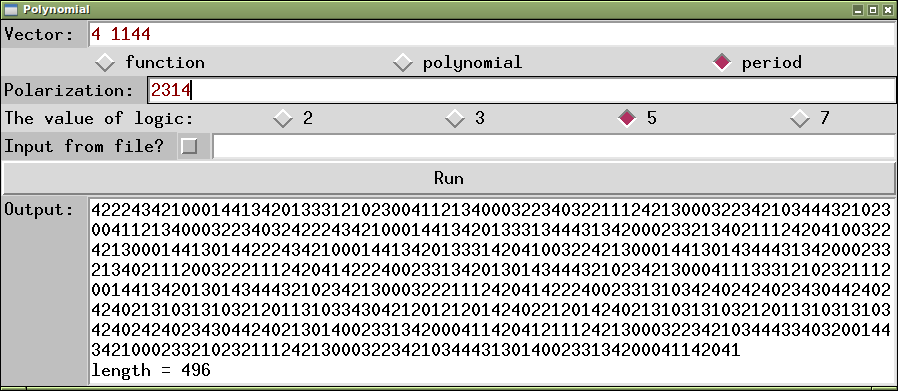
\includegraphics[width=0.95\textwidth]{polyscreen.png}
    \caption{Вид интерфейса \label{ps}}
    \end{figure}
\item Программа на языке \ttfamily{C++}, осуществляющая для заданного числа пременных $n$
    "быстрый"{} поиск функций длина которых, в классе пляризованных полиномов, больше заданного
    порога, среди заданного класса симметрических функций от $n$ переменных;
\item С помощью системы компьютерной алгебры \ttfamily{Sage} \cite{sage} были произведены: получение
    полиномиальных форм, поляризованных по разным векторам поляризации и подстановка значений в
    полиномы для проверки правильности их построения.
\end{itemize}
Коды всех программ доступны в моем репозитории, располеженном по адресу:
\mbox{\url{https://www.github.com/obirvalger/diploma}}.



\newpage
\tableofcontents

\makeatletter
\renewcommand*{\@biblabel}[1]{\hfill#1.}
\makeatother

\newpage
% \cleardoublepage

\begin{thebibliography}{0}
\bibitem{ue04} Угрюмов~Е.\,П. Цифровая схемотехника. СПб.: БХВ-Петербург, 2004.
\bibitem{sb90} Sasao T., Besslich P. On the complexity of mod-2 sum PLA’s  // IEEE Trans.on Comput. 39. N 2. 1990. P.~262--266. 
\bibitem{sv93} Супрун~В.\,П. Сложность булевых функций в классе канонических поляризованных полиномов // Дискретная математика. 5.
    \textnumero 2. 1993. С. 111--115. 
\bibitem{pn95} Перязев Н.\,А. Сложность булевых функций в классе полиномиальных поляризованных~форм // Алгебра и логика. 34.
    \textnumero 3. 1995. С. 323--326. 
\bibitem{ss02} Селезнева С.\,H. О сложности представления функций многозначных логик поляризованными полиномами. Дискретная
    математика. 14. \textnumero 2. 2002. С.~48--53.
\bibitem{kk05} Кириченко~К.\,Д. Верхняя оценка сложности полиномиальных нормальных форм булевых функций 
    // Дискретная математика. 17. \textnumero 3. 2005. С. 80--88.
\bibitem{sd08} Селезнева С.\,Н. Дайняк А.\,Б. О сложности обобщенных полиномов k\nobreakdash-значных функций // Вестник Московского
    университета. Серия 15. Вычислительная математика и кибернетика. \textnumero 3. 2008. С. 34--39.
\bibitem{mn12} Маркелов Н.\,К. Нижняя оценка сложности функций трехзначной логики в классе поляризованных полиномов // Вестник
    Московского университета. Серия 15. Вычислительная математика и кибернетика. \textnumero 3. 2012. С. 40--45.
\bibitem{sm09} Селезнева С.\,H. Маркелов Н.\,К. Быстрый алгоритм построения векторов коэффициэнтов поляризованных полиномов
    k-значных функций // Ученые записки Казанского университета. Серия Физико-математические науки. 2009. 151.
    \textnumero 2 С.~147-151.
\bibitem{sage} [Sage] William A. Stein et al., Sage Mathematics Software (Version 6.4).
    The Sage Development Team, 2015, \url{http://www.sagemath.org}.
 
\end{thebibliography}

\end{document}
